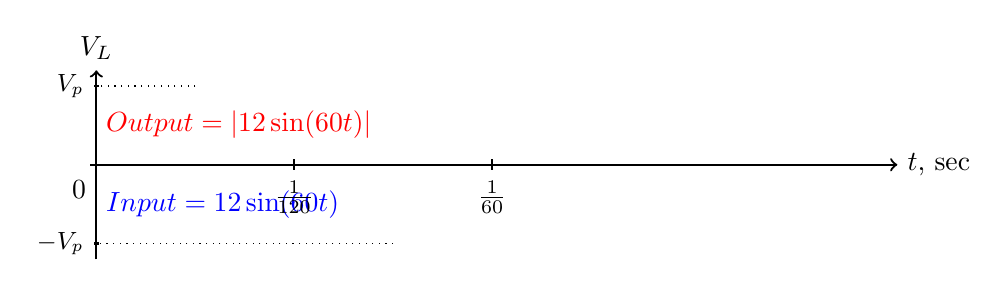
\begin{tikzpicture}[domain=0:8*pi, xscale=.4]
    %\draw[very thin,color=gray] (-0.1,-1.1) grid (8*pi, 1.1);
    \draw[->, thick] (-0.2,0) -- (8*pi+.3,0) node[right] {$t$, sec};
    \draw[->, thick] (0,-1.2) -- (0,1.2) node[above] {$V_L$};
    \draw[color=blue, smooth] plot[id=sin] function{sin(.5 * x)}
        node[below right, yshift=-.5\baselineskip] {$\text{Input} = 12 \sin(60 t)$};
    \draw[color=red, dashed] plot[id=abs-sin] function{abs(sin(.5 * x))}
        node[above right, yshift=.5\baselineskip] {$\text{Output} = \left| 12 \sin(60 t) \right|$};

	% vertical axis values
	\draw[dotted] (pi, 1) -- (0, 1);
	\draw[thick] (2pt, 1) -- (-2pt, 1) node[anchor=east] {\small$V_p$};

	\draw[dotted] (3*pi, -1) -- (0, -1);
	\draw[thick] (2pt, -1) -- (-2pt, -1) node[anchor=east] {\small$-V_p$};

	% tics
	\draw[thick] (0, 2pt) -- (0, -2pt) node[anchor=north east] {0};
	\draw[thick] (2*pi, 2pt) -- (2*pi, -2pt) node[anchor=north] {$\frac{1}{120}$};
	\draw[thick] (4*pi, 2pt) -- (4*pi, -2pt) node[anchor=north] {$\frac{1}{60}$};
\end{tikzpicture}
